\section{Protocolli di Sicurezza}

Un protocollo di sicurezza è una sequenza di azioni (passi) che
coinvolge due o più parti,
finalizzata all'instaurazione di una comunicazione sicura tra di esse,
al sicuro dalle azioni di un
possibile intruso. L'insieme dei passi specificati costituisce la sessione
del protocollo.
Servono per garantire l'autenticità dell'utente.

\paragraph{Nonce: }
In crittografia il termine nonce indica un numero, generalmente casuale
o pseudo-casuale,
che ha un utilizzo unico. Nonce deriva infatti dall'espressione inglese
``for the nonce'', che significa
appunto ``per l'occasione''. Un nonce viene utilizzato spesso nei protocolli
di autenticazione per
assicurare che i dati scambiati nelle vecchie comunicazioni non possano
essere utilizzati in
attacchi di tipo replay attack.\\

\paragraph{La spia DY:}
In tutti i protocolli di autenticazione che analizzeremo di seguito, viene identificata la possibilità che vi sia una ``spia'' (intruder) all'interno del sistema che può effettuare una serie di operazioni, quali:
\begin{itemize}
    \item Intercettare messaggi e prevenirne il recapito;
    \item Far rimbalzare a piacere i messaggi intercettati;
    \item Imparare i testi in chiaro e i testi codificati;
    \item Tentare di decriptare con tutte le chiavi note;
    \item Utilizzare le proprie credenziali legali;
    \item Ottenere certe credenziali illegalmente;
    \item Creare messaggi fasulli da componenti già note;
\end{itemize}

\section[Autenticazione di utenti remoti con Needham-Schr\"{o}der
(1978)]{Autenticazione di utenti remoti\\ con Needham-Schr\"{o}der (1978)}

Sono stati definiti vari protocolli a riguardo. L'obiettivo è quello di
garantire l'autenticazione
dell'utente da remoto appunto, ottenuta dallo scambio segreto dei nonce.
Needham-Schröder è basato sulla crittografia asimmetrica e permette
di assicurare la mutua
autenticazione tra due entità di rete. Nella sua forma proposta
non è sicuro.
Utilizzeremo dei messaggi fatti così:

\begin{itemize}
    \item Nomi di utenti: \(A\), \(B\), \(C\), \(\ldots \)
    \item Chiavi crittografiche
          \begin{itemize}
              \item a lungo termine: \(K_a\), \(K_b\), \(\ldots \)
              \item a breve termine: \(K_{ab}\),  \(\ldots \) (chiavi di sessione)
          \end{itemize}
    \item Nonce: \(N_a\), \(N_b\), \(\ldots \)
    \item Timestamp: \(T_a\), \(T_b\), \(\ldots \)
    \item Digest
    \item Label: ``trasferisci denaro'', ``collegati alla porta xy'', \(\ldots \)
\end{itemize}

I messaggi base possono essere a loro volta composti:
\begin{itemize}
    \item Concatenati: \(m, m', \ldots\)
    \item Criptati: \(m_K\), \(\{m,m'\}_K\), \(\ldots\)
\end{itemize}

Il protocollo presuppone una PKI (infrastruttura a chiave pubblica)
con crittografia perfetta.

\begin{figure}[H]
    \centering
    \includegraphics[width=10cm, keepaspectratio]{capitoli/crittografia/imgs/alieno.png}
\end{figure}

Alice vuole identificarsi con Bob, quindi Bob alla fine dell'applicazione del protocollo dovrà essere
sicuro di aver comunicato con Alice.
\begin{enumerate}
    \item Alice invia un messaggio a Bob, criptato con la
          chiave pubblica di quest'ultimo e che quindi solo lui potrà aprire, in cui inserisce chi lo sta contattando ed un nonce. Il nonce \(N_a\) permette di capire se il messaggio che è stato inviato è nuovo. Si analizzano tutti i nonce già utilizzati per verificare che esso sia appunto un valore mai visto;
    \item Bob riceve il messaggio e lo apre. Una volta
          letto, risponde ad Alice: invia indietro il nonce
          \(N_a\) ricevuto, più ne aggiunge uno nuovo,  \(N_b\), questa volta per fare in modo che sia lui ad autenticarsi con Alice. Il messaggio è codificato con la chiave pubblica di Alice, \(K_{alice}\);
    \item Alice riceve la risposta e invia a sua volta
          \(N_b\) a Bob. A questo punto Bob è sicuro di poter
          parlare con Alice.
\end{enumerate}

L'autenticazione è garantita dal fatto che i nonce non
possono necessariamente avere lo stesso
numero e che le chiavi a lungo termine non possono
essere compromesse.
La prova del fatto che il messaggio 1 sia stato inviato
da Alice ci viene data dalla chiave \(K_{alice}\) nel
messaggio 2 e quindi sappiamo che solo lei lo può aprire.

\subsection{Attacco di Lowe (1995)}

Uno studente di Cambridge, Lowe, dimostra che il protocollo appena visto non
funziona perché è possibile attaccarlo. Ciò significa che qualcun altro potrebbe
riuscire a spacciarsi per Alice con Bob (in riferimento all'esempio precedente).

\begin{figure}[H]
    \centering
    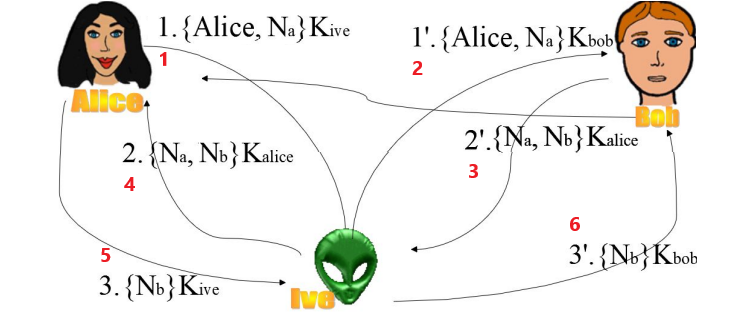
\includegraphics[width=\textwidth, keepaspectratio]{capitoli/crittografia/imgs/alienospinning.png}
\end{figure}

\paragraph{Nel Dettaglio: }
Ive è uno dei partecipanti al protocollo:

\begin{enumerate}
    \item[1.]  Alice vuole comunicare con lei. Ive (che però è l'intruder)
        apre il messaggio inviato da Alice
        (grazie alla sua chiave privata) e lo invia a Bob;
    \item[1'.] Ive, che vuole spacciarsi per Alice nei confronti di Bob,
        ricodifica il messaggio prima di inoltrarlo
        a Bob;
    \item[2'.] Bob segue le regole del protocollo N-S ed invia ad Alice
        \(\{N_a, N_b\}\) criptato con \(K_{alice}\). Ive
        potrebbe lasciare andare il messaggio oppure
    \item[2.] potrebbe intercettarlo e rispedirlo ad Alice.
\end{enumerate}
Tutti i partecipanti, nel momento in cui ricevono dei messaggi, devono
verificare che gli invii
corrispondano a quanto specificato nel protocollo. Se così non fosse, tutta
l'esecuzione cadrebbe e
verrebbe riavviata da zero.

\begin{enumerate}
    \item[2.] Il messaggio inviato da Ive ad Alice ha come primo
        elemento \(N_a\) (il nonce di Alice), e come secondo elemento \(N_b\)
        (il nonce di Bob) che Alice crede sia stato
        generato da Ive;
    \item[3.] Alice inoltra \(N_b\) ad Ive criptando con la chiave di Ive, \(K_{ive}\);
    \item[3'.] Ive apre il messaggio e lo invia a Bob, criptato con \(K_{bob}\)
\end{enumerate}

Bob, che è l'utente di cui il protocollo si approfitta, riceve \(N_b\).
Controlla che il nonce sia quella che
ha effettivamente inventato e a quel punto è sicuro di parlare con Alice.
Ive ha quindi usato il nonce che ha inventato Alice per approfittarsi di
Bob. Ha effettuato un
\textit{attacco di autenticazione}, in quanto Bob pensa di comunicare con
Alice, ma in realtà sta parlando
con Ive.
Ive si spaccerà per Alice con Bob visto che si è autenticata al suo posto,
quindi può chiedergli dei
servizi. Per esempio, se Bob rappresentasse una banca, Ive potrebbe
richiedere un trasferimento
di denaro dal conto di Alice al proprio.
Lo stesso tipo di attacco può essere studiato nella tassonomia BUG. Tale
soluzione è deprecata
ma continua ad essere utilizzata.
Sappiamo che Alice ha condiviso con Ive il nonce \(N_a\) da lei generato, ma
questo in realtà è stato
inoltrato anche a Bob. Bob, nel caso in cui avesse delle intenzioni
malevole, potrebbe utilizzare \(N_a\)
ai danni di Alice: se Alice vedesse arrivare un messaggio contenente \(N_a\)
e \(N_b\), infatti, penserebbe
che questo sia stato inviato da Ive. Bob però, conoscendo l'importanza di
\(N_a\), potrebbe agire,
stavolta vendicandosi su Ive.
Il protocollo presenta delle vulnerabilità, quindi non è del tutto sicuro.
Per ovviare a questo
problema, si potrebbe aggiungere una comunicazione fuori banda. Ogni qual
volta un utente voglia
autenticarsi, prima di eseguire una sua qualunque istruzione, è necessario
verificarne l'effettiva
identità.

\section{Protocollo di sicurezza di Woo-Lam (anni 80)}

Usa la crittografia simmetrica e usa un TTP (Trusted Third Party), che
possiede un database di
tutte le chiavi. Un TTP è un'entità che facilita le interazioni tra due
parti che si fidano entrambe
della ``terza parte''.
L'obiettivo del protocollo è che Alice (\(A\)) riesca ad autenticarsi
con Bob (\(B\)).

\begin{figure}[H]
    \centering
    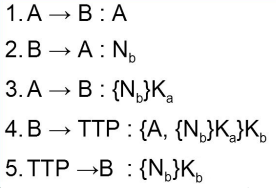
\includegraphics[width=7cm, keepaspectratio]{capitoli/crittografia/imgs/Mulan.png}
\end{figure}

\begin{enumerate}
    \item A invia un messaggio pubblico a B;
    \item B invia ad A un nonce \(N_b\) per verificare che stia
          effettivamente comunicando con lei. Anche questo messaggio è
          pubblico;
    \item A riceve \(N_b\) e lo inoltra di risposta a Bob, ma criptata con
          \(K_a\). \(K_a\) è una chiave simmetrica che ha in condivisione con il
          TTP e che B non può aprire. Bob deve verificare che \(K_a\)
          appartenga davvero ad A;
    \item B invia la richiesta al TTP di aprire il messaggio per verificare
          l'appartenenza di \(K_a\). Il messaggio è criptato con \(K_b\) e lo
          può aprire solo il TTP poiché condivide le chiavi simmetriche con B;
    \item Il TTP, una volta decifrato il messaggio e ottenuto \(N_b\), lo
          inoltra a B. B apre il messaggio finale perché possiede \(K_b\) e
          verifica che \(N_b\) sia il nonce che ha inviato ad A. Se è così,
          significa che B ha effettivamente comunicato con A. La decodifica di
          \(\{N_b\}_{K_a}\) funziona solo se \(K_a\) appartiene ad A.
\end{enumerate}

\subsection{Attacco su Woo-Lam}

Anche detto ``interlacciamento di sessioni''.
\begin{figure}[H]
    \centering
    \includegraphics[width=8cm, keepaspectratio]{capitoli/crittografia/imgs/mulan2.png}
\end{figure}
\begin{enumerate}
    \item[1.] C'è l'attaccante C che si vuole spacciare per A con
        B e invia un messaggio a B confermando ciò;
    \item[1'.] C invia anche un altro messaggio a B dove
        afferma invece di essere C; Alla ricezione dei due
        messaggi, B segue il protocollo e genera due nonce;
    \item[2.] In risposta ad A genera \(N_b\);
    \item[2'.] In risposta a C genera \(N_b'\);
        C intercetta i messaggi e quindi anche i due nonce.
    \item[3/3'.] C invia \(N_b\) criptato con \(K_c\) a B due volte;
        B quindi riceve lo stesso messaggio due volte.
    \item[4.] Supponendo che un messaggio sia stato inviato
        da A, B invia al TTP il nonce \(N_b\) che ha ricevuto. Il
        messaggio è poi criptato con \(K_b\);
    \item[4'.] B invia un altro messaggio al TTP ma questa
        volta con C all'interno.
    \item[5.] TTP invia a B il nonce \(N_b''\) ottenuto a partire dalla
        decifratura del messaggio 4 (nonce completamente
        sbagliato);
    \item[5'.] TTP invia a B il nonce \(N_b\) ottenuto a partire dalla
        decifratura del messaggio 4'
\end{enumerate}

B aveva associato ad A il nonce \(N_b\) quindi quando gli verrà ritornato penserà che è stato inviato da A. B andrà allora ad autenticare C al posto di A. Inoltre, se B attiva due comunicazioni contemporaneamente non può sapere in che ordine arriveranno i messaggi a causa del funzionamento di HTTP, quindi si potrebbe vedere ricevere prima il nonce ``corretto'' (quello inviato da TTP per C nel messaggio 4') invece che quello ``corrotto'' (inviato da TTP per A nel messaggio 4).\\

Il protocollo Woo-Lam è quindi vulnerabile. Per risolvere teoricamente basta che il TTP inserisca nel messaggio di ritorno quello che è l'utente per il quale ha decifrato il nonce.\\

Si porta all'attenzione dell'egregio lettore che esiste anche la versione
simmetrica di Needham-Schröder (questa è un informazione dalla
dubbia utilità).